%%%%%%%%%%%%%%%%%%%%%%%%%%%%%%%%%%%%%%%%%
% Journal Article
% LaTeX Template
% Version 1.4 (15/5/16)
%
% This template has been downloaded from:
% http://www.LaTeXTemplates.com
%
% Original author:
% Frits Wenneker (http://www.howtotex.com) with extensive modifications by
% Vel (vel@LaTeXTemplates.com)
%
% License:
% CC BY-NC-SA 3.0 (http://creativecommons.org/licenses/by-nc-sa/3.0/)
%
%%%%%%%%%%%%%%%%%%%%%%%%%%%%%%%%%%%%%%%%%

%----------------------------------------------------------------------------------------
%	PACKAGES AND OTHER DOCUMENT CONFIGURATIONS
%----------------------------------------------------------------------------------------

\documentclass[twoside, twocolumn]{article}

\usepackage{blindtext} % Package to generate dummy text throughout this template 

\usepackage[sc]{mathpazo} % Use the Palatino font
\usepackage[T1]{fontenc} % Use 8-bit encoding that has 256 glyphs
\linespread{1.05} % Line spacing - Palatino needs more space between lines
\usepackage{microtype} % Slightly tweak font spacing for aesthetics

\usepackage[english]{babel} % Language hyphenation and typographical rules

\usepackage[hmarginratio=1:1,top=32mm,columnsep=20pt]{geometry} % Document margins
\usepackage[hang, small,labelfont=bf,up,textfont=it,up]{caption} % Custom captions under/above floats in tables or figures
\usepackage{booktabs} % Horizontal rules in tables

\usepackage{lettrine} % The lettrine is the first enlarged letter at the beginning of the text

\usepackage{amsmath}
\usepackage{graphicx}

\usepackage{enumitem} % Customized lists
\setlist[itemize]{noitemsep} % Make itemize lists more compact

\usepackage{abstract} % Allows abstract customization
\renewcommand{\abstractnamefont}{\normalfont\bfseries} % Set the "Abstract" text to bold
\renewcommand{\abstracttextfont}{\normalfont\small\itshape} % Set the abstract itself to small italic text

\usepackage{titlesec} % Allows customization of titles
\renewcommand\thesection{\Roman{section}} % Roman numerals for the sections
\renewcommand\thesubsection{\roman{subsection}} % roman numerals for subsections
\titleformat{\section}[block]{\large\scshape\centering}{\thesection.}{1em}{} % Change the look of the section titles
\titleformat{\subsection}[block]{\large}{\thesubsection.}{1em}{} % Change the look of the section titles

\usepackage{fancyhdr} % Headers and footers
\pagestyle{fancy} % All pages have headers and footers
\fancyhead{} % Blank out the default header
\fancyfoot{} % Blank out the default footer
\fancyhead[C]{Project 1 $\bullet$ Borries, Thiel $\bullet$ WS 2016/17} % Custom header text
\fancyfoot[RO,LE]{\thepage} % Custom footer text

\usepackage{titling} % Customizing the title section

\usepackage{hyperref} % For hyperlinks in the PDF

%----------------------------------------------------------------------------------------
%	TITLE SECTION
%----------------------------------------------------------------------------------------

\setlength{\droptitle}{-4\baselineskip} % Move the title up

\pretitle{\begin{center}\Huge\bfseries} % Article title formatting
\posttitle{\end{center}} % Article title closing formatting
\title{Machine Learning - Deep Learning Project 1} % Article title
\author{%
\textsc{Anton Borries} \\[1ex] 
\normalsize 2204600 \\
\normalsize  \href{mailto:anton.borries@hhu.de}{anton.borries@hhu.de}
\and 
\textsc{Johannes Thiel} \\[1ex]
\normalsize 2164216 \\ 
\normalsize \href{mailto:johannes.thiel@hhu.de}{johannes.thiel@hhu.de} 
}

\date{\today} % Leave empty to omit a date
\renewcommand{\maketitlehookd}{%
\begin{abstract}
\noindent We train a neural Network to recognize Images from the MNIST Dataset. The Accuracy only reaches $98.9\%$ due to Hardware constraints during training.
\end{abstract}
}

%----------------------------------------------------------------------------------------

\begin{document}

% Print the title
\maketitle

%----------------------------------------------------------------------------------------
%	ARTICLE CONTENTS
%----------------------------------------------------------------------------------------

\section{Architecture}

\lettrine[nindent=.2em,lines=3]{O} ur Network consists out of 4 total Layers. The first two are both Convolutional Layers and the second ones are both Fully Connected. \\
We used ReLu as our Activation Function for all Layers.

\begin{table}[htb]
\label{table_conv}
	\caption{Convolutional Layers}
	\centering
		\begin{tabular}{l l l l}
			Layer & 1 & 2 \\
			\midrule
			Input Size & 28 x 28 & 14 x 14 \\
			Filter Size & 5 x 5 & 5 x 5 \\
			Output Channels & 32 & 64 \\
			Pooling & 2 x 2 & 2 x 2 \\
			Activation Function & ReLu & ReLu \\
\end{tabular}
\end{table}

\begin{table}[htb]
\label{table_fcl}
	\caption{Fully Connected Layers}
	\centering
		\begin{tabular}{l l l l}
			Layer & 3 & 4 \\
			\midrule
			Input Size & 7 x 7 x 64 & 1024 \\
			Activation Function & ReLu & ReLu \\
			Dropout & Yes & No \\
\end{tabular}
\end{table}

%------------------------------------------------

\section{Training}

We used a Batch Size of 128 to train our Network. \\
For the loss function we decided on using the cross entropy method.

\begin{equation}
 C = - \dfrac{1}{n} \sum_{z} [y \ln a + (1 - y) \ln (1 - a)]
\end{equation}

This is helping us, avoiding the learning slowdown \cite{crossentro}.\\
We utilized the Adam Optimizer with a learning rate of $0.001$ to train the Network. \\
We decided on training for 1000 Epochs because of Hardware restrains.

%------------------------------------------------

\section{Evaluation}
We reached a performance of $98.9\%$.\\
This score was calculated by validating against the MNIST Test data.\\
We are aware that this is a relativly low accuracy given our architecure.\\
If we would have trained the Network for a longer time or with more Epochs in general we are certain that we would score better.\\
Nevertheless this is still a higher score than the Network in Exercise 2 which scored about $96\%$.\\


%------------------------------------------------

\section{Randomness}

The results differ from run to run although only slightly. This is due to the fact that all weights are initialized randomly (Standard deviation of $0.1$).

%------------------------------------------------

\section{Optimization iterations}

All training was performed on on a Intel i5-4299U @ 1,60GHz x4 CPU.

\begin{table}[htb]
\label{table_opt}
	\caption{Optimization Iterations}
	\centering
		\begin{tabular}{l l l}
			No. of Epochs & Accuracy & Duration \\
			\midrule
			100 & 0.9578 & 5 min 26 sec\\
			300 & 0.9747 & 15 min 09 sec\\
			1000 & 0.98.9 & 50 min 59 sec\\
\end{tabular}
\end{table}

We can see that the time it takes to tain the network is linear to the number of epochs.

%------------------------------------------------

\section{Change of learning rate}

A higher learning rate helps us learn faster in the beginnig. In later stages though, this leads to the results changing in variance rather drastically.\\
Smaller learnings rates on the other hand are leading to a smaller increase in results for each epoch. However with more epochs they will get better as well. This is backed by our Network getting better the more epochs we use for training.\\
Also this proves that our Network would probably perform better if we trained for a longer time.

%------------------------------------------------

\section{Visualization}
Roughly put, the Network is learning to detect Edges and their orientations.\\
Some Examples show the following.\\
\begin{figure}[htb]
\centering
	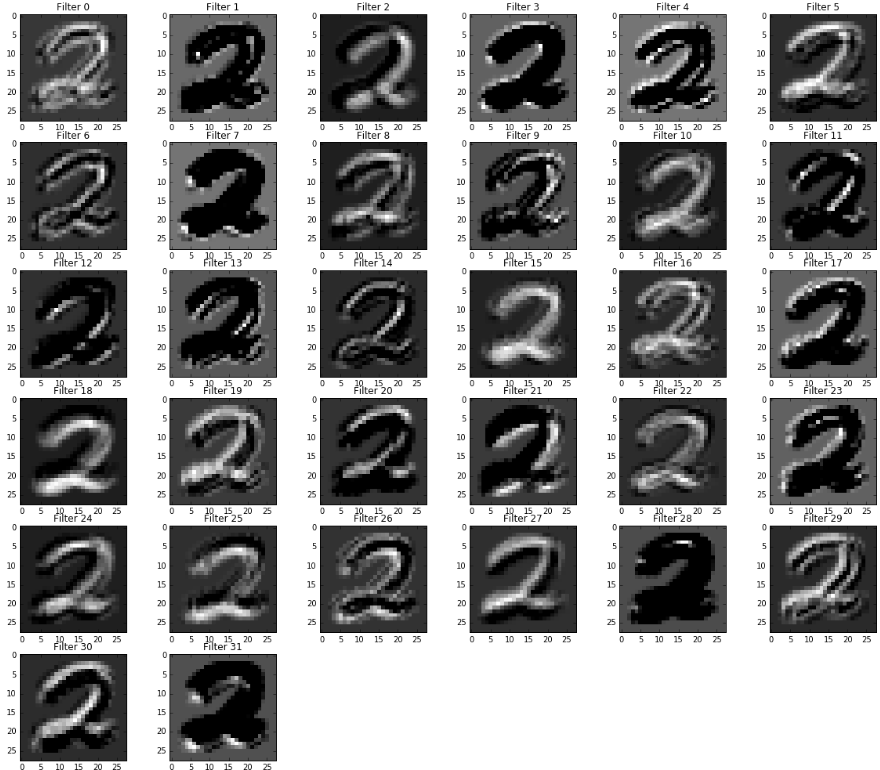
\includegraphics[width=0.48\textwidth]{activations.png}
	\caption{Example of Activations in Layer 1}
\end{figure}
\begin{itemize}
 \item Filter 2 is detecting right facing Edges
 \item Filter 5 is detecting left facing Edges
 \item Filter 6 is detecting outer bounds
 \item Filter 25 is detecting bottom facing Edges
\end{itemize}





%------------------------------------------------

\section{Configuration changes}

Training with 100 epochs. We tried changing the batch size.

\begin{table}[htb]
\label{table_batch}
	\caption{Changing the Batch size}
	\centering
		\begin{tabular}{l l l}
			Batch Size & Accuracy \\
			\midrule
			256 & 0.933\\
			512 & 0.944\\
			1024 & 0.975\\
			2048 & 0.976\\
\end{tabular}
\end{table}

As you can see. The Batch Size had no effect after reaching 1024
Changing the amount of Filters lead to no difference in the results.

%------------------------------------------------

\section{Minimum Configuration}

Of course a definition for a minimum configuration is always dependand on how you would define "good results".\\
We created a Network with only two Layers.\\
The first is a Convolutional Layer with 32 5 x 5 Filters using 4 x 4 Pooling. The second Layer is a Fully Connected Layer with 127 Neurons.\\
Training this Network with a Batch Size of 100 lead to a accuracy of $95\%$ which is in the same order as our complete Network. 

%------------------------------------------------

\section{No Pooling}
Taking away the pooling in the Convolutional Layers led to two effects.\\
\begin{itemize}
	\item Training was way slower. On our machine it was almost slower by a factor of 10
	\item Accuracy went down to $92\%$
\end{itemize}

%----------------------------------------------------------------------------------------
%	REFERENCE LIST
%----------------------------------------------------------------------------------------

\begin{thebibliography}{99} % Bibliography - this is intentionally simple in this template

\bibitem{crossentro}Cross Entropy,\\ \url{http://neuralnetworksanddeeplearning.com/chap3.html}, 06 12 2016.
 
\end{thebibliography}

%----------------------------------------------------------------------------------------

\end{document}
